\documentclass{standalone}
\usepackage{tikz}
\usepackage{ctex,siunitx}
\usepackage{tkz-euclide}
\usepackage{amsmath}
\usetikzlibrary{patterns, calc}
\usetikzlibrary {decorations.pathmorphing, decorations.pathreplacing, decorations.shapes,decorations.markings,positioning, snakes}

\begin{document}
\small
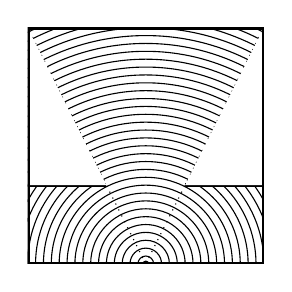
\begin{tikzpicture}[>=stealth]
  \clip (-1.5, 0) rectangle (1.5,3);
  \foreach \x in {.1,.2,...,5}
  {
      \draw (-\x,0) arc (180:0:\x);
  }
  % \fill [white](-5.1,-2) rectangle (-1.5, 6);
  % \fill [white](1.5,-2) rectangle (5.1, 6);
  \draw[ultra thick] (-1.5,1)--(-.5,1);
  \draw[ultra thick] (1.5,1)--(.5,1);
  \draw [dotted](0,0)--(-.5,1)--(-1,2)--(-1.5,3);
  \draw [dotted](0,0)--(.5,1)--(1,2)--(1.5,3);
  % \fill [white](-1.5,3) rectangle (1.5, 6);
  \fill [white](-1.5,1)--(-.5,1)--(-1.5,3)--(-1.5,1);
  \fill [white](1.5,1)--(.5,1)--(1.5,3)--(1.5,1);
  \draw [ultra thick](-1.5, 0) rectangle (1.5,3);
  \draw  [fill=black] (0,0)  circle (1pt);
\end{tikzpicture}
\end{document}